\documentclass[a4paper, 12pt]{article}
\usepackage{vntex}
\usepackage{a4wide,amssymb,epsfig,latexsym,array,hhline,fancyhdr}
\usepackage[normalem]{ulem}
\usepackage[makeroom]{cancel}
\usepackage{amsmath}
\usepackage{longtable}
\usepackage{amsthm}
\usepackage{multicol,longtable,amscd}
\usepackage{diagbox}%Make diagonal lines in tables
\usepackage{booktabs}
\usepackage{alltt}
\usepackage[framemethod=tikz]{mdframed}% For highlighting paragraph backgrounds
\usepackage{caption,subcaption}
\usepackage{lastpage}
\usepackage[lined,boxed,commentsnumbered]{algorithm2e}
\usepackage{enumerate}
\usepackage{color}
\usepackage{xcolor}
\usepackage{graphicx}							% Standard graphics package
\usepackage{array}
\usepackage{tabularx, caption}
\usepackage{multirow}
\usepackage{multicol}
\usepackage{rotating}
\usepackage{graphics}
\usepackage{geometry}
\usepackage{setspace}
\usepackage{epsfig}
\usepackage{tikz}
\usepackage{listings}
\usepackage{float}
\usetikzlibrary{arrows,snakes,backgrounds}
\usepackage{hyperref}
\hypersetup{urlcolor=black,linkcolor=black,citecolor=black,colorlinks=true} 
%\usepackage{pstcol} 								% PSTricks with the standard color package

\newtheorem{theorem}{{\bf Theorem}}
\newtheorem{property}{{\bf Property}}
\newtheorem{proposition}{{\bf Proposition}}
\newtheorem{corollary}[proposition]{{\bf Corollary}}
\newtheorem{lemma}[proposition]{{\bf Lemma}}

\AtBeginDocument{\renewcommand*\contentsname{Mục lục}}
\AtBeginDocument{\renewcommand*\refname{Tài liệu tham khảo}}
\AtBeginDocument{\renewcommand*\listfigurename{Tiêu đề ảnh}}
%\usepackage{fancyhdr}
\setlength{\headheight}{40pt}
\pagestyle{fancy}
\fancyhead{} % clear all header fields
\fancyhead[L]{
 \begin{tabular}{rl}
    \begin{picture}(25,15)(0,0)
    \put(0,-8){
\includegraphics[width=8mm, height=8mm]{hcmut.png}}
   \end{picture}&
	\begin{tabular}{l}
		\textbf{\bf \ttfamily Trường Đại Học Bách Khoa Tp.Hồ Chí Minh}\\
		\textbf{\bf \ttfamily Khoa Khoa Học \& Kỹ Thuật Máy Tính}
	\end{tabular} 	
 \end{tabular}
}
\fancyhead[R]{
	\begin{tabular}{l}
		\tiny \bf \\
		\tiny \bf 
	\end{tabular}  }
\fancyfoot{} % clear all footer fields
\fancyfoot[L]{\scriptsize \ttfamily Báo cáo môn Kiểm tra phần mềm - Học kì 241}
\fancyfoot[R]{\scriptsize \ttfamily Trang {\thepage}/\pageref{LastPage}}
\renewcommand{\headrulewidth}{0.3pt}
\renewcommand{\footrulewidth}{0.3pt}


%%%
\setcounter{secnumdepth}{4}
\setcounter{tocdepth}{3}
\makeatletter
\newcounter {subsubsubsection}[subsubsection]
\renewcommand\thesubsubsubsection{\thesubsubsection .\@alph\c@subsubsubsection}
\newcommand\subsubsubsection{\@startsection{subsubsubsection}{4}{\z@}%
                                     {-3.25ex\@plus -1ex \@minus -.2ex}%
                                     {1.5ex \@plus .2ex}%
                                     {\normalfont\normalsize\bfseries}}
\newcommand*\l@subsubsubsection{\@dottedtocline{3}{10.0em}{4.1em}}
\newcommand*{\subsubsubsectionmark}[1]{}
%\renewcommand{\thesubsubsection}{\alph{subsubsection}}
\everymath{\color{blue}}
\makeatother

\begin{document}

\begin{titlepage}
\begin{center}
VIETNAM NATIONAL UNIVERSITY, HO CHI MINH CITY \\
UNIVERSITY OF TECHNOLOGY \\
FACULTY OF COMPUTER SCIENCE AND ENGINEERING
\end{center}
\vspace{1cm}

\begin{figure}[h!]
\begin{center}

\includegraphics[width=3cm]{hcmut.png}
\end{center}
\end{figure}

\vspace{1cm}


\begin{center}
\begin{tabular}{c}
\multicolumn{1}{l}{\textbf{{\Large KIỂM TRA PHẦN MỀM (CO3015)}}}\\

~~\\
\hline
\\
\\
\textbf{{\Huge BTL 2: BLACK BOX TESTING}}\\
\\

\\
\hline
\end{tabular}
\end{center}

\vspace{3cm}

\begin{table}[h]
\begin{tabular}{rrl}
\hspace{3 cm} & Giảng viên hướng dẫn: & Bùi Hoài Thắng\\

& Sinh viên thực hiện:
& Phạm Đức Hào - 2111128\\
&& Hồ Trọng Nhân - 2111899\\
&& Đậu Đức Quân - 2114531\\
&& Nguyễn Phúc Minh Quân - 2110479\\
&& Trần Mậu Thật - 2112342
\end{tabular}
\end{table}

\begin{center}
{\footnotesize HO CHI MINH CITY, NOVEMBER 2024}
\end{center}
\end{titlepage}


\newpage
\tableofcontents
\newpage
\section{Giới thiệu:}

\section{Phân công}
 \begin{table}[H]
\centering
\begin{tabular}{|p{3cm}|p{3cm}|l|c|}
\hline 
Reviewer &
Validator &
  \multicolumn{1}{c|}{Feature} &Contributon \\ \hline
Đậu Đức Quân & Trần Mậu Thật &&\\\hline
Hồ Trọng Nhân & Đậu Đức Quân &Private Messaging, Private File Upload&\\ \hline
Nguyễn Phúc Minh Quân & Hồ Trọng Nhân &&\\ \hline
Phạm Đức Hào & Nguyễn Phúc Minh Quân &&\\ \hline
Trần Mậu Thật & Phạm Đức Hào &&\\ \hline
\end{tabular}
\caption{Bảng phân công công việc}
\label{tab:my-table}
\end{table}





\newpage
\section{Quá trình làm việc nhóm:}
\subsection{Buổi họp trao đổi những thắc mắc của các thành viên về bài tập lớn và phân công công việc. (15/11/2024)}
Nội dung chính:
\begin{itemize}
    \item Thảo luận về nội dung bài tập lớn.
    \item Thảo luận cách phân công công việc cho từng thành viên.
\end{itemize}
Kết quả cuộc họp:
\begin{itemize}
  \item Mỗi thành viên đã hiểu rõ nhiệm vụ của mình.
  \item Xác định được deadline và buổi meet sync kế tiếp.
\end{itemize}

\subsection{Buổi họp đồng bộ tiến độ làm việc của các thành viên. (22/11/2024)}
Nội dung chính:
\begin{itemize}
    \item Mỗi thành viên trình bày công việc đã làm được và khó khăn cần sự trợ giúp.
    \item Mỗi thành viên review công việc của thành viên khác.
\end{itemize}
Kết quả cuộc họp:
\begin{itemize}
    \item Mỗi thành viên đã hoàn thành công việc của mình.
    \item Bản báo cáo đã được hoàn thiện và sẵn sàng nộp. 
\end{itemize}

\newpage

\section{Kết quả kiểm thử}

\subsection{Tính năng 1}
\subsubsection{Mô tả}
\subsubsection{Test case}
\subsection{Tính năng 2}

\subsection{Chức năng Tạo sự kiện (Create event)}
\subsubsection{Use case}
\begin{table}[H]
    \centering
    \begin{tabular}{|l|p{11cm}|}
        \hline
        Category & Description \\
        \hline
        Use case name & Create event\\
        \hline
        Actor & Manager \\
        \hline
        Assumption & Người dùng ở trang \url{https://sandbox.moodledemo.net/}. Ngôn ngữ trang web được chỉnh tiếng Việt. Người dùng đăng nhập thành công dưới bất kì tài khoản nào. Người dùng đang ở trang "Bảng điều khiển". \\
        \hline
        Normal flow & 1. Người dùng nhấn vào nút "Sự kiện mới". \\
        & 2. Hệ thống hiển thị bảng "Sự kiện mới". \\
        & 3. Người dùng nhập thông tin có thể bao gồm chữ, số và kí tự vào ô "Tên sự kiện". \\
        & 4. Người dùng chọn thông tin ngày, tháng, năm, giờ, phút của sự kiện. \\
        & 5. Người dùng chọn "Thành viên" hoặc "Hệ thống" tại hàng "Loại sự kiện".\\
        & 6. Người dùng nhấn vào nút "Lưu". \\
        & 7. Hệ thống đóng bảng "Sự kiện mới". \\
        \hline
        Alternative flows & A1. Tại bước 6: \\
        & 6.1. Người dùng nhấn vào nút "Show more". \\
        & 6.2. Người dùng nhập thông tin vào ô "Mô tả". \\
        & Quay lại bước 6 trên Normal flow. \\
        & \\
        & A2. Tại bước 6: \\
        & 6.1. Người dùng nhấn vào nút "Show more". \\
        & 6.2. Người dùng nhập thông tin vào ô "Địa chỉ". \\
        & Quay lại bước 6 trên Normal flow. \\
        & \\
        & A3. Tại bước 6: \\
        & 6.1. Người dùng nhấn vào nút "Show more". \\
        & 6.2. Người dùng chọn lựa chọn "Tới" tại hàng "Thời lượng". \\
        & 6.3. Người dùng chọn thông tin ngày, tháng, năm, giờ, phút kết thúc của sự kiện. \\
        & Quay lại bước 6 trên Normal flow. \\
        & \\
        & A4. Tại bước 6: \\
        & 6.1. Người dùng nhấn vào nút "Show more". \\
        & 6.2. Người dùng chọn lựa chọn "Thời lượng tính bằng phút" tại hàng "Thời lượng". \\
        & 6.3. Người dùng nhập thông tin vào ô dưới "Thời lượng tính bằng phút". \\
        & Quay lại bước 6 trên Normal flow. \\
        & \\
        & A5. Tại bước 6: \\
        & 6.1. Người dùng nhấn vào nút "Show more". \\
        & 6.2. Người dùng chọn vào ô "Lặp lại sự kiện này". \\
        & 6.3. Người dùng nhập thông tin vào ô "Lặp lại hàng tuần, tạo ra tất cả". \\
        & Quay lại bước 6 trên Normal flow. \\
        & \\
        & A6. Tại bước 5: \\
        & 5.1. Người dùng chọn "Mục" tại hàng "Loại sự kiện". \\
        & 5.2. Người dùng chọn các mục cần thiết tại hàng "Mục". \\
        & Quay lại bước 6 trên Normal flow. \\
        \hline
        Exception flows & \\
        & E1. Tại bước 3: \\
        & 3.1. Người dùng không nhập vào ô "Tên sự kiện". \\
        & 3.2. Người dùng nhấn nút "Lưu". \\
        & 3.3. Hệ thống báo lỗi "Bắt buộc". \\
        & Quay lại bước 3 trên Normal flow. \\
        & \\
        & E2. Tại bước 6: \\
        & 6.1. Người dùng nhấn vào nút "Show more". \\
        & 6.2. Người dùng chọn lựa chọn "Thời lượng tính bằng phút" tại hàng "Thời lượng". \\
        & 6.3. Người dùng nhập thông tin không phải số nguyên dương vào ô dưới "Thời lượng tính bằng phút". \\
        & 6.4. Người dùng nhấn nút "Lưu". \\
        & 6.5. Hệ thống báo lỗi "Khoảng thời gian tính bằng phút mà bạn vừa nhập không có hiệu lực. Vui lòng nhập một khoảng thời gian tính bằng phút lớn hơn 0 hoặc không chọn thời gian.". \\
        & Quay lại bước 6.2 trên Alternative flow A4. \\
        & \\
        & E3. Tại bước 6: \\
        & 6.1. Người dùng nhấn vào nút "Show more". \\
        & 6.2. Người dùng chọn lựa chọn "Tới" tại hàng "Thời lượng". \\
        & 6.3. Người dùng chọn thông tin ngày, tháng, năm, giờ, phút kết thúc của sự kiện diễn ra trước thời điểm bắt đầu. \\
        & 6.4. Người dùng nhấn vào nút "Lưu". \\
        & 6.5. Hệ thống báo lỗi "Khoảng thời gian ngày và giờ bạn chọn diễn ra trước khi sự kiện bắt đầu. Vui lòng điều chỉnh trước khi tiếp tục.". \\
        & Quay lại bước 6.3 trên Alternative flow A3. \\
        & \\
        E4. Tại bước 5: \\
        & 5.1. Người dùng chọn "Mục" tại hàng "Loại sự kiện". \\
        & 5.2. Người dùng xóa hết các mục tại hàng "Mục". \\
        & 5.3. Người dùng nhấn vào nút "Lưu". \\
        & 5.4. Hệ thống báo lỗi "Hãy chọn một chuyên mục". \\
        & Quay lại bước 5.2 trên Alternative flow A6. \\
        \hline
    \end{tabular}
    \caption{Use case: Create event}
    \label{Use case: Create event}
\end{table}
\subsubsection{Activity diagram}
\subsubsection{Sử dụng phương pháp Boundary value analysis để kiểm thử}
\subsubsection{Sử dụng phương pháp Equivalence class partitioning}
\subsubsection{Sử dụng phương pháp Decision table để kiểm thử}
\subsubsection{Sử dụng phương pháp Use-case testing để kiểm thử}

\subsection{Chức năng Đổi mật khẩu (Change password)}
\subsubsection{Use case}
\begin{table}[H]
    \centering
    \begin{tabular}{|l|p{11cm}|}
        \hline
        Category & Description \\
        \hline
        Use case name & Change password \\
        \hline
        Actor & Người dùng \\
        \hline
        Assumption & Người dùng ở trang \url{https://sandbox.moodledemo.net/}. Ngôn ngữ trang web được chỉnh tiếng Việt. Người dùng đăng nhập thành công dưới bất kì tài khoản nào. Người dùng đang ở trang "Trang chủ". \\
        \hline
        Normal flow & 1. Người dùng nhấn vào nút mũi tên góc phải trên ngay bên cạnh hình đại diện. \\
        & 2. Người dùng nhấn vào "Tùy chọn". \\
        & 3. Người dùng nhấn vào "Đổi mật khẩu". \\
        & 4. Người dùng nhập đúng mật khẩu hiện tại vào ô "Mật khẩu hiện hành".\\
        & 5. Người dùng nhập mật khẩu mới có thể bao gồm cả chữ, số, kí tự vào ô "Mật khẩu mới".\\
        & 6. Người dùng nhập chính xác thông tin đã nhập ở ô "Mật khẩu mới" vào ô "Mật khẩu mới (lại)".\\
        & 7. Người dùng nhấn vào nút "Lưu những thay đổi". \\
        \hline
        Alternative flows & Không có. \\
        \hline
        Exception flows & E1. Tại bước 4: \\
        & 4.1. Người dùng không nhập thông tin ở nội dung "Mật khẩu hiện hành". \\ 
        & Thực hiện tiếp tục bước 5. Sau khi thực hiện bước 7, hệ thống sẽ hiển thị lỗi "Bắt buộc". Quay lại bước 4 trên Normal flow. \\
        & \\
        & E2. Tại bước 5: \\
        & 5.1. Người dùng không nhập thông tin ở nội dung "Mật khẩu mới". \\
        & Thực hiện tiếp tục bước 6. Sau khi thực hiện bước 7, hệ thống sẽ hiển thị lỗi "Bắt buộc". Quay lại bước 5 trên Normal flow. \\
        & \\
        & E3. Tại bước 6: \\
        & 6.1. Người dùng không nhập thông tin ở nội dung "Mật khẩu mới (lại)". \\
        & Thực hiện tiếp tục bước 7. Sau khi thực hiện bước 7, hệ thống sẽ hiển thị lỗi "Bắt buộc". Quay lại bước 6 trên Normal flow. \\
        & \\
        & E4. Tại bước 4: \\
        & 4.1. Người dùng nhập nhập thông tin tại ô "Mật khẩu hiện hành" chưa chính xác. \\
        & Thực hiện tiếp tục bước 5. Sau khi thực hiện bước 7, hệ thống sẽ hiển thị lỗi "Đăng nhập sai, xin vui lòng thử lại". Quay lại bước 4 trên Normal flow. \\
        & \\
        & E5. Tại bước 6 : \\
        & 6.1. Người dùng nhập nhập thông tin tại ô "Mật khẩu mới (lại)" chưa khớp với nội dung đã nhập tại ô "Mật khẩu mới". \\
        & Thực hiện tiếp tục bước 7. Sau khi thực hiện bước 7, hệ thống sẽ hiển thị lỗi "Các mật khẩu không trùng khớp". Quay lại bước 5 trên Normal flow. \\
        \hline
    \end{tabular}
    \caption{Use case: Change password}
    \label{Use case: Change password}
\end{table}
\subsubsection{Activity diagram}
\subsubsection{Sử dụng phương pháp Boundary value analysis để kiểm thử}
\subsubsection{Sử dụng phương pháp Equivalence class partitioning}
\subsubsection{Sử dụng phương pháp Decision table để kiểm thử}
\subsubsection{Sử dụng phương pháp Use-case testing để kiểm thử}

\subsection{Chức năng Tạo bài kiểm tra (Create quiz)}
\subsubsection{Use case}

\begin{table}[H]
    \centering
    \begin{tabular}{|l|p{11cm}|}
        \hline
        Category & Description \\
        \hline
        Use case name & Create quiz \\
        \hline
        Actor & Giáo viên \\
        \hline
        Assumption & Người dùng đang ở đường dẫn \url{https://sandbox.moodledemo.net/}. Ngôn ngữ của trang web được chỉnh là Tiếng Việt. Người dùng đăng nhập thành công dưới tài khoản giáo viên. Người dùng đang ở trang "Trang chủ". Có ít nhất một khoá học.\\\hline
        Normal flow & 
        1. Người dùng chọn Khoá học cần tạo bài kiểm tra. \\
        & 2. Người dùng bật "Chế độ chỉnh sửa" ở góc phải trên trang web. \\
        & 3. Người dùng chọn "Thêm một hoạt động hoặc tài nguyên" ở section phù hợp.\\
        & 4. Người dùng chọn "Trắc nghiệm" từ danh sách các hoạt động.\\
        & 5. Người dùng thiết lập các thông số cho bài kiểm tra.\\
        & 6. Người dùng nhấn "Lưu và trở về khoá học" và quay về trang chính của khoá học.\\
        & 7. Người dùng chọn thẻ bài kiểm tra vừa tạo.\\
        & 8. Người dùng chọn "Thêm câu hỏi" để thêm câu hỏi vào bài kiểm tra.\\\hline
        Alternative flows &
        A1. Tại bước 6:\\
        & 6.1. Người dùng chọn "Lưu và cho xem" và được điều hướng đến trang "Thêm câu hỏi".\\
        & Thực hiện tiếp tục bước 8 trên Normal flow.\\
        \\\hline
        Exception flows &
        E1. Tại bước 5:\\
        & 5.1. Người dùng không nhập tên bài kiểm tra.\\
        & Thực hiện tiếp tục bước 6. Hệ thống sẽ hiển thị lỗi "You must supply a value here.". Quay lại bước 5 trên Normal flow.\\\hline
    \end{tabular}
    \caption{Use case: Create quiz}
    \label{tab:create-quiz}
\end{table}

\subsubsection{Activity diagram}
\subsubsection{Sử dụng phương pháp Boundary value analysis để kiểm thử}
Ta chọn Normal Boundary Value testing, thay đổi input ở bước 5 dựa theo domain như sau:
\begin{itemize}
    \item "Tên": Gồm các ký tự in được. Ký hiệu độ dài là $x$, ta có $1 \leq x$. Để phù hợp với thực tế, ta cũng set giá trị $x$ tối đa là 200. Tóm lại, ta có $1 \leq x \leq 200$.
\end{itemize}

\subsubsection{Sử dụng phương pháp Equivalence class partitioning}
Thực hiện Weak Normal Equivalence Class Testing, chia input ở bước 5 thành các equivalence class như sau:
\begin{itemize}
    \item "Tên": Giống như ở phần Boundary Value Testing, ta chia thành 1 class: $1 \leq x \leq 200$.
\end{itemize}
\subsubsection{Sử dụng phương pháp Decision table để kiểm thử}

\begin{table}[H]
    \centering
    \begin{tabular}{|p{5cm}|c|c|c|c|}
        \hline
        \textbf{Điều kiện} & \textbf{1} & \textbf{2} & \textbf{3} & \textbf{4} \\
        \hline
        c1. Đã bật chế độ chỉnh sửa & Có & Có & Không & Không \\
        \hline
        c2. Đã nhập tên bài kiểm tra hợp lệ ($1 \leq x \leq 200$) & Có & Không & Có & Không \\
        \hline
        \hline
        \textbf{a1. Cho phép tạo bài kiểm tra} & x & & & \\
        \hline
        \textbf{a2. Hiển thị lỗi yêu cầu nhập tên bài kiểm tra} & & x & & \\
        \hline
        \textbf{a3. Không hiển thị chỗ tạo bài} & & & x & x \\
        \hline
        \textbf{a4. Không hợp lệ} & & &x & \\\hline
    \end{tabular}
    \caption{Bảng quyết định kiểm thử chức năng tạo bài kiểm tra}
    \label{tab:decision-table-create-quiz}
\end{table}

\subsubsection{Sử dụng phương pháp Use-case testing để kiểm thử}

\subsection{Chức năng Nhắn tin (Send message)}
\subsubsection{Use case}

\begin{table}[H]
    \centering
    \begin{tabular}{|l|p{11cm}|}
        \hline
        Category & Description \\
        \hline
        Use case name & Send message \\
        \hline
        Actor & Sinh viên \\
        \hline
        Assumption & Người dùng đang ở đường dẫn \url{https://sandbox.moodledemo.net/}. Ngôn ngữ của trang web được chỉnh là Tiếng Việt. Người dùng đăng nhập thành công dưới tài khoản sinh viên. Người dùng đang ở trang "Trang chủ".\\\hline
        Normal flow & 
        1. Người dùng toggle menu ở góc trái trên trang web. \\
        & 2. Người dùng chọn mục "Tin nhắn" ở menu. \\
        & 3. Người dùng tìm kiếm tên của người cần nhắn tin.\\
        & 4. Người dùng nhập nội dung tin nhắn vào ô "Write a message".\\
        & 5. Người dùng bấm ký tự gửi tin nhắn.\\\hline
        Alternative flows &
        A1. Tại bước 1:\\
        & 1.1. Người dùng chọn ký tự message trên header.\\
        & Thực hiện tiếp tục bước 3 trên Normal flow.\\
        \\\hline
        Exception flows &
        E1. Tại bước 3:\\
        & 3.1. Người dùng không tìm thấy tên người cần nhắn.\\
        & Thực hiện lại bước 3, kiểm tra chính tả. Sau khi tìm thấy người cần nhắn thì tiếp tục bước 4 trên Normal flow.\\\hline
    \end{tabular}
    \caption{Use case: Send message}
    \label{tab:send-message}
\end{table}

\subsubsection{Activity diagram}
\subsubsection{Sử dụng phương pháp Boundary value analysis để kiểm thử}
Ta chọn Normal Boundary Value testing, thay đổi input ở bước 4 dựa theo domain như sau:
\begin{itemize}
    \item "Nội dung": Gồm các ký tự in được. Ký hiệu độ dài là $x$, ta có $1 \leq x$. Để phù hợp với thực tế, ta cũng set giá trị $x$ tối đa là 500. Tóm lại, ta có $1 \leq x \leq 500$.
\end{itemize}

\subsubsection{Sử dụng phương pháp Equivalence class partitioning}
Thực hiện Weak Normal Equivalence Class Testing, chia input ở bước 5 thành các equivalence class như sau:
\begin{itemize}
    \item "Tên": Giống như ở phần Boundary Value Testing, ta chia thành 1 class: $1 \leq x \leq 500$.
\end{itemize}
\subsubsection{Sử dụng phương pháp Decision table để kiểm thử}

\begin{table}[H]
    \centering
    \begin{tabular}{|l|c|c|c|c|}
        \hline
        \textbf{Điều kiện} & \textbf{1} & \textbf{2} & \textbf{3} & \textbf{4} \\
        \hline
        c1. Người dùng tìm thấy tên người cần nhắn & Có & Không & Có & Không \\
        \hline
        c2. Nội dung tin nhắn hợp lệ ($1 \leq x \leq 500$) & Có & Có & Không & Không \\\hline
        \hline
        \textbf{a1. Cho phép gửi tin nhắn} & x & & & \\
        \hline
        \textbf{a2. Không hiển thị kết quả tìm kiếm} & & x & &x \\
        \hline
        \textbf{a3. Hiển thị lỗi nội dung tin nhắn} & & &x & \\\hline
        \textbf{a4. Không hợp lệ} & &x & & \\
        \hline
    \end{tabular}
    \caption{Bảng quyết định kiểm thử chức năng nhắn tin}
    \label{tab:decision-table}
\end{table}

\subsubsection{Sử dụng phương pháp Use-case testing để kiểm thử}

\newpage
\subsection{Chức năng tải file riêng tư (Private file upload)}
\subsubsection{Use case}

\begin{table}[H]
    \centering
    \begin{tabular}{|l|p{11cm}|}
        \hline
        Category & Description \\
        \hline
        Use case name & Private file upload \\
        \hline
        Actor & Sinh viên \\
        \hline
        Assumption & Người dùng đang ở đường dẫn \url{https://school.moodledemo.net/}. Ngôn ngữ của trang web được chỉnh là Tiếng Việt. Người dùng đăng nhập thành công dưới tài khoản sinh viên. Người dùng đang ở trang "Trang chủ".\\\hline
        Normal flow & 
        1. Ở trang chủ, người dùng nhấn chọn vào biểu tượng avatar người dùng. \\
        & 2. Người dùng chọn “Tập tin riêng tư”. \\
        & 3. Hệ thống hiển thị trang tải tập tin.\\
        & 4. Người dùng chọn vào icon “Thêm…” để thêm.\\
        & 5. Người dùng chọn “Choose file”.\\
        & 6. Hệ thống hiển thị cửa sổ chọn file.\\
        & 7. Người dùng chọn file cần tải lên.\\
        & 8. Người dùng chọn “Đăng tải tệp này”.\\
        & 9. Người dùng chọn “Lưu những thay đổi”.\\
        & 10. File được upload thành công.\\\hline
        Alternative flows &
        A1. Tại bước 4:\\
        & 4.1. Người dùng nhấn vào vùng “Thêm các tập tin bằng cách kéo thả”.\\
        & Người dùng tiếp tục thực hiện theo bước 5.\\
        & A2. Tại bước 4:\\
        & 4.1. Người dùng kéo thả file vào vùng “Thêm các tập tin bằng cách kéo thả”.\\
        & Người dùng tiếp tục thực hiện theo bước 9.
        \\\hline
        Exception flows &
        E1. Tại bước 7:\\
        & 7.1 Người dùng chọn file < 1 byte hoặc > 100MB.\\
        & 7.2 Người dùng chọn “Đăng tải tệp này”.\\
        & Hệ thống sẽ báo lỗi kích thước file.\\\hline
    \end{tabular}
    \caption{Use case: Private file upload}
    \label{tab:private-file-upload}
\end{table}

\subsubsection{Activity diagram}
\begin{figure}[H]
    \centering
    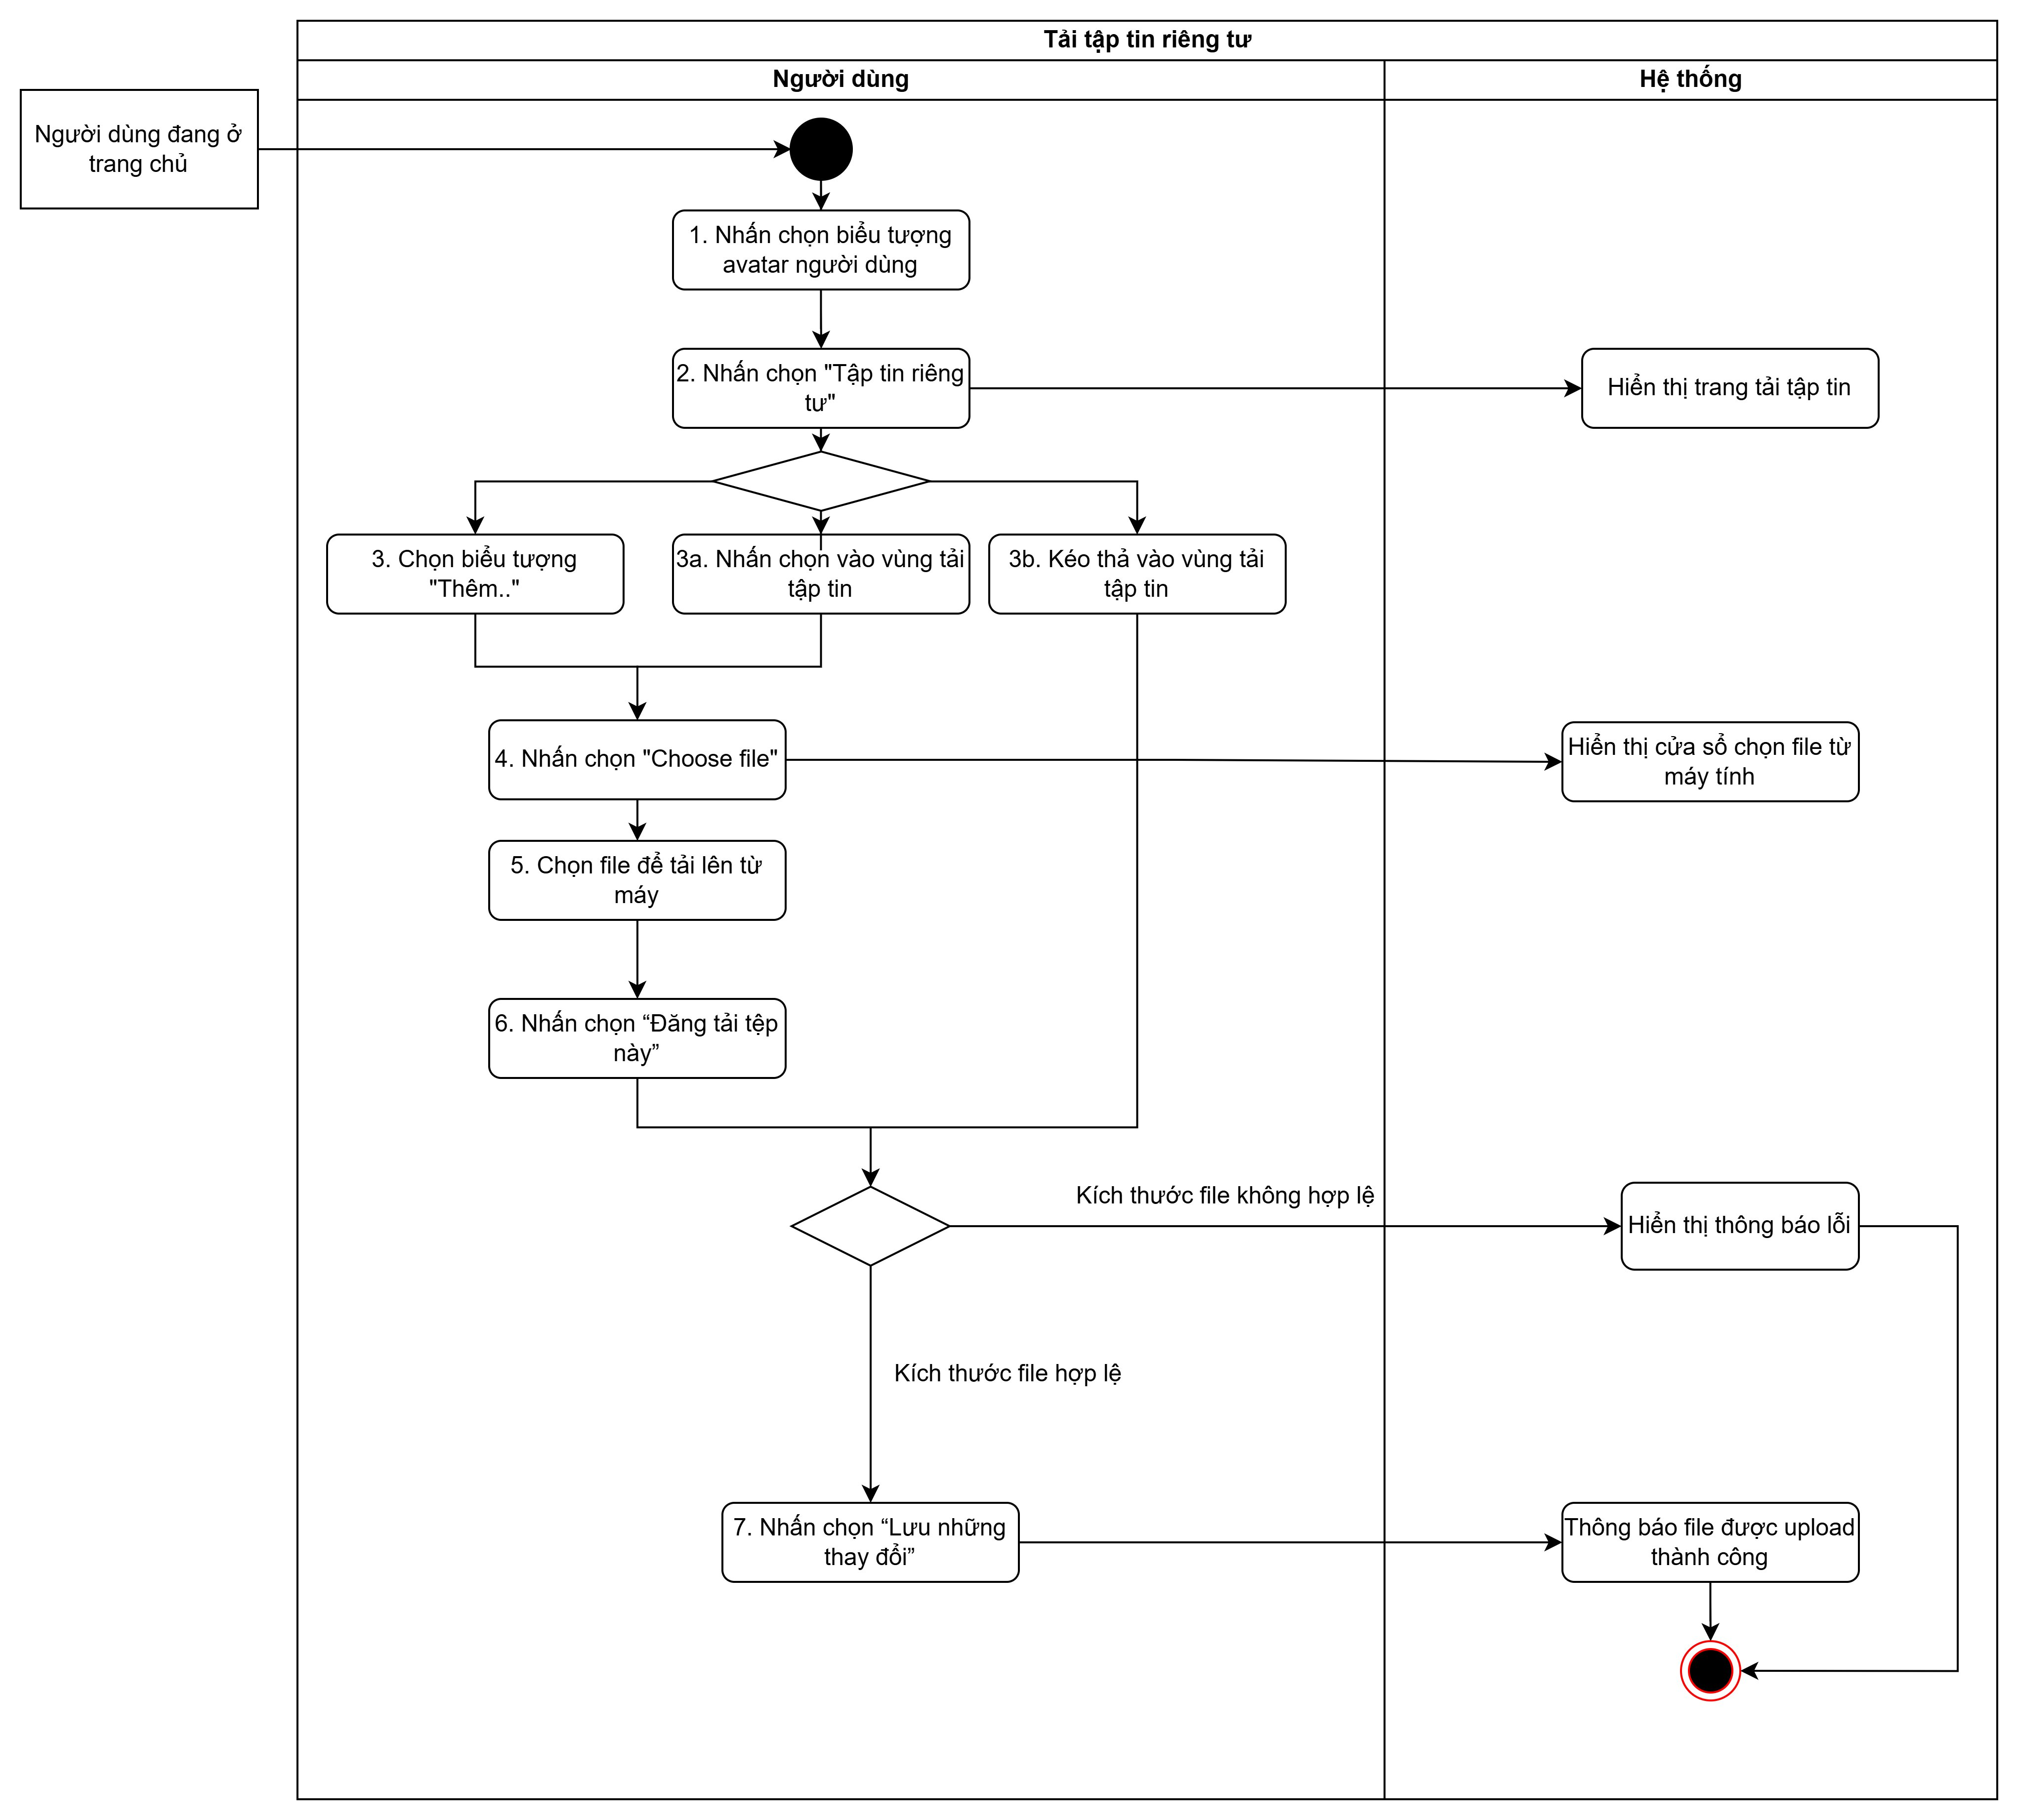
\includegraphics[width=\textwidth]{image/private-file-upload.png}
    \caption{Activity diagram for Private file upload}
    \label{fig:activity-diagram-private-file-upload}
\end{figure}
\subsubsection{Sử dụng phương pháp Boundary value analysis để kiểm thử}
Ta chọn Normal Boundary Value testing, dựa theo các lí do sau:
\begin{itemize}
    \item Kích thước file upload là 1 phạm vi liên tục với biên rõ ràng, lựa chọn BVA phù hợp để kiểm thử các giá trị tại biên, gần biên.
    \item Kiểm tra giá trị biên giúp đảm bảo rằng hệ thống xử lý đúng các tình huống cận biên, nơi dễ phát sinh lỗi nhất.
\end{itemize}
Thay giá trị input ở bước 7 theo domain như sau, gọi x là "Kích thước của file upload" \(1\ \text{byte} \leq x \leq 100\text{MB}\).
\begin{itemize}
    \item PF-001-001: Upload file kích thước giữa 1 byte - 100MB.
    \item PF-001-002: Upload file kích thước nhỏ nhất cho phép.
    \item PF-001-003: Upload file kích thước nhỏ nhất cho phép +.
    \item PF-001-004: Upload file kích thước lớn nhất cho phép -.
    \item PF-001-005: Upload file kích thước lớn nhất cho phép.
\end{itemize}
\subsubsection{Sử dụng phương pháp Equivalence class partitioning}
Lí do chọn: Chức năng upload file dựa trên một phạm vi kích thước liên tục rõ ràng (1 byte - 100 MB). Có thể dễ dàng chia ra lớp tương đương hợp lệ và không hợp lệ. \\
Thực hiện Weak Normal Equivalence Class Testing, chia input ở bước 7 thành các equivalence class như sau:
\begin{itemize}
    \item "Kích thước file" gọi là x, ta chia thành 1 class valid: \(1\ \text{byte} \leq x \leq 100\text{MB}\), 2 class invalid là \(x < 1\ \text{byte}\) và \(x > 100\text{MB}\).
\end{itemize}
Test case:
\begin{itemize}
    \item PF-002-001: Upload file kích thước < 1 byte.
    \item PF-002-002: Upload file kích thước > 100MB
    \item PF-001-001: Upload file kích thước giữa 1 byte - 100MB.
\end{itemize}

\subsubsection{Sử dụng phương pháp Use-case testing để kiểm thử}
Dựa theo Activity diagram, ta chia thành các path:
\begin{itemize}
    \item P1: 1,2,3,4,5,6,7 tương ứng với PF-001-001
    \item P2: 1,2,3a,4,5,6,7 tương ứng với PF-003-001
    \item P3: 1,2,3b,7 tương ứng với PF-003-002
    \item  P4: 1,2,3b tương ứng với PF-003-003
\end{itemize}
\newpage
\subsection{Chức năng nhắn tin riêng tư (Private message)}
\subsubsection{Use case}

\begin{table}[H]
    \centering
    \begin{tabular}{|l|p{11cm}|}
        \hline
        Category & Description \\
        \hline
        Use case name & Private message \\
        \hline
        Actor & Sinh viên \\
        \hline
        Assumption & Người dùng đang ở đường dẫn \url{https://school.moodledemo.net/}. Ngôn ngữ của trang web được chỉnh là Tiếng Việt. \\ 
        & - User 1 username: amandahamilto205, password: moodle\\
        & - User 2 username: student, password: moodle\\
        &Người dùng đăng nhập thành công dưới tài khoản sinh viên. Người dùng đang ở trang "Trang chủ".\\\hline
        Normal flow & 
        1. Ở trang chủ, user 1 click biểu tượng Chat. \\
        & 2. Hệ thống hiển thị khung chat nhỏ trên màn hình. \\
        & 3. User 1 chọn user 2 trong mục Riêng tư trên khung chat nhỏ.\\
        & 4. Hệ thống hiển thị lịch sử chat.\\
        & 5. User 1 gõ tin nhắn văn bản, icon vào ô chat và nhấn gửi.\\
        & 6. Hệ thống hiển thị tin nhắn user 1 vừa gửi trên chatbox.\\
        & 7. Hệ thống gửi tin nhắn và hiển thị thông báo đến user 2.\\\hline
        Alternative flows &
        A1. Tại bước 5:\\
        & 5.1 Người dùng nhấn chọn tin nhắn.\\
        & 5.2 Người dùng chọn icon Xóa những tin nhắn được chọn.\\
        & 5.3 Người dùng xác nhận Xóa.
        \\\hline
        Exception flows &
        E1. Tại bước 5:\\
        & 5.1 Người dùng gửi tin nhắn với độ dài 4100 kí tự.\\
        & 5.2 Hệ thống giới hạn độ dài tin nhắn 4096 kí tự và không có phép gõ nữa.\\ & \\
        & E2. Tại bước 6, nếu user 2 đã block user 1\\
        & 6.1: Hệ thống hiển thị lỗi không gửi được tin nhắn cho user 2.\\\hline
    \end{tabular}
    \caption{Use case: Private message}
    \label{tab:Private-message}
\end{table}

\subsubsection{Activity diagram}
\begin{figure}[H]
    \centering
    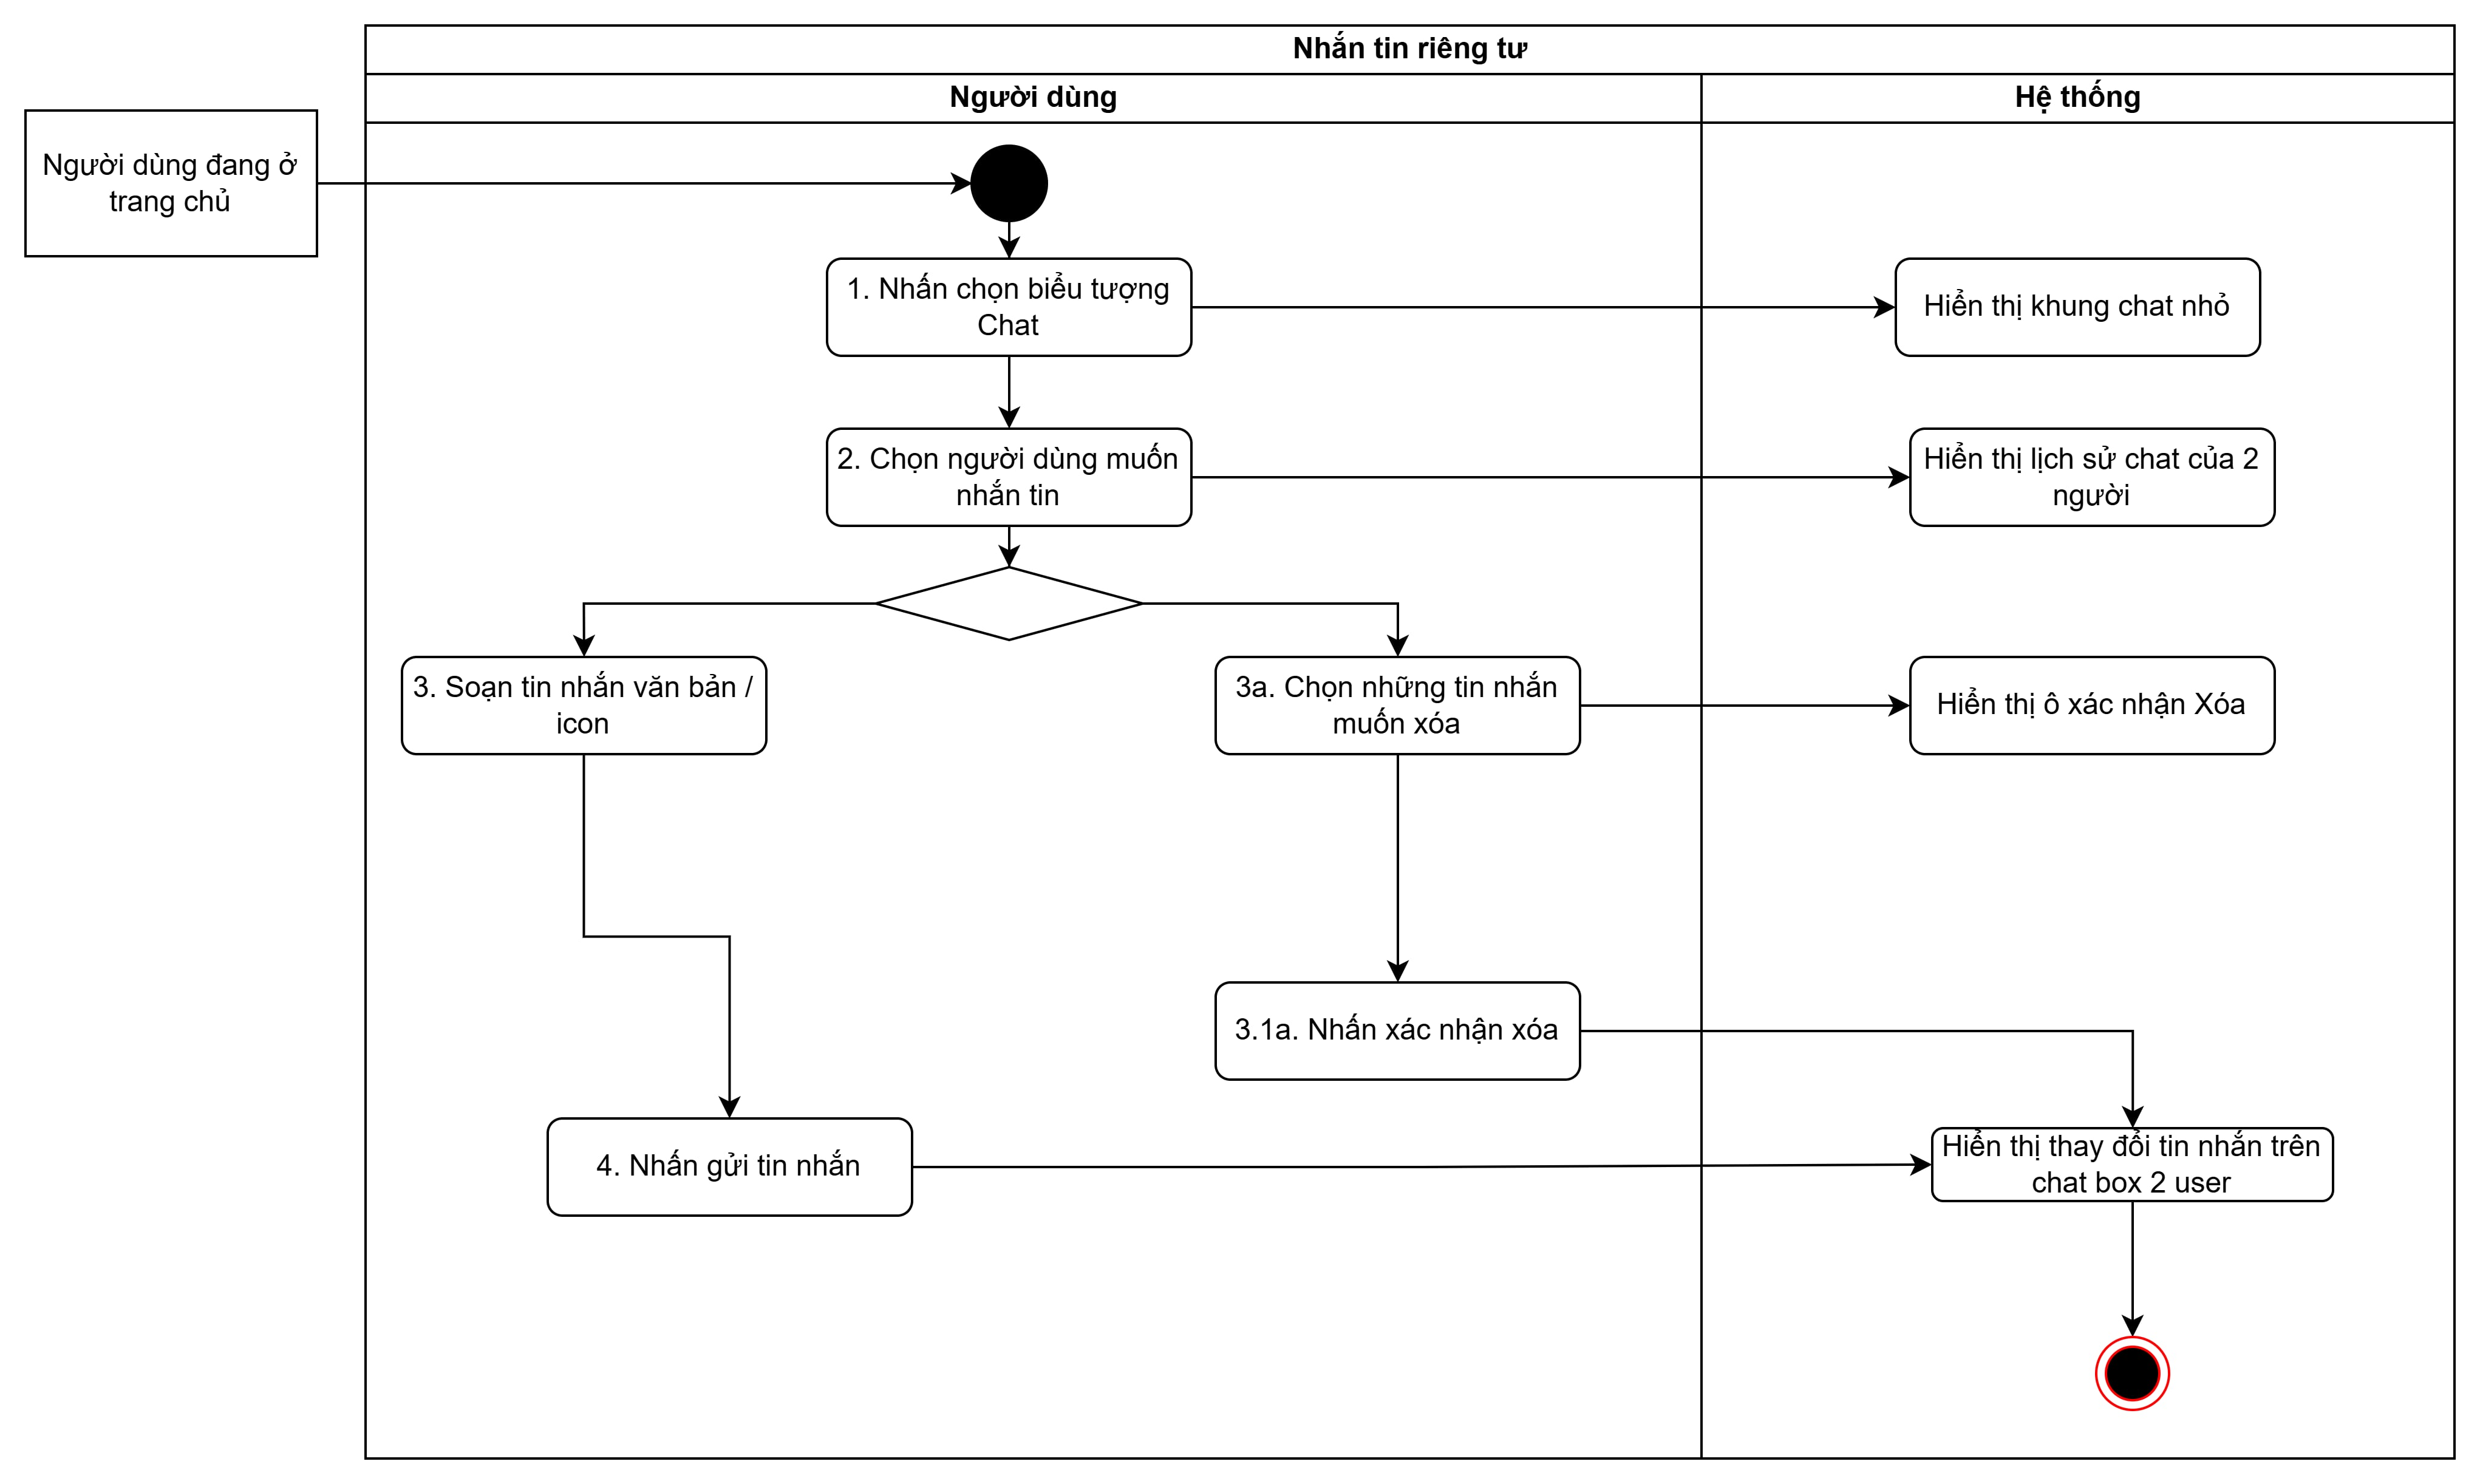
\includegraphics[width=\textwidth]{image/private-message.png}
    \caption{Activity diagram for Private message}
    \label{fig:activity-diagram-private-message}
\end{figure}
\subsubsection{Sử dụng phương pháp Boundary value analysis để kiểm thử}
Ta chọn Normal Boundary Value testing, dựa theo các lí do sau:
\begin{itemize}
    \item Giới hạn số lượng kí tự tin nhắn là 1 phạm vi liên tục với biên rõ ràng, lựa chọn BVA phù hợp để kiểm thử các giá trị tại biên, gần biên.
    \item Kiểm tra giá trị biên giúp đảm bảo rằng hệ thống xử lý đúng các tình huống cận biên, nơi dễ phát sinh lỗi nhất.
\end{itemize}
Thay giá trị input ở bước 5 theo domain như sau, gọi x là "Số lượng kí tự input" \(1\ \text{kí tự} \leq x \leq 4096\ \text{kí tự}\).
\begin{itemize}
    \item PM-001-001: Gửi tin nhắn với số lượng kí tự từ 1 - 4096.
    \item PM-001-002: Gửi tin nhắn với số lượng kí tự tối thiểu.
    \item PM-001-003: Gửi tin nhắn với số lượng kí tự tối thiểu +.
    \item PM-001-004: Gửi tin nhắn với số lượng kí tự tối đa.
    \item PM-001-005: Gửi tin nhắn với số lượng kí tự tối đa -.
\end{itemize}
\subsubsection{Sử dụng phương pháp Equivalence class partitioning}
Lí do chọn: Chức năng gửi tin nhắn riêng tư có số lượng kí tự giới hạn dựa trên một phạm vi kích thước liên tục rõ ràng (1 kí tự - 4096 kí tự). Có thể dễ dàng chia ra lớp tương đương hợp lệ và không hợp lệ.. \\
Thực hiện Weak Normal Equivalence Class Testing, chia input ở bước 5 thành các equivalence class như sau:
\begin{itemize}
    \item "Số lượng kí tự" gọi là x, ta chia thành 1 class valid: \(1\ \text{kí tự} \leq x \leq 4096\ \text{kí tự}\), 2 class invalid là \(x < 1\ \text{kí tự}\) và \(x > 4096\ \text{kí tự}\).
\end{itemize}
Test case:
\begin{itemize}
    \item PM-002-001: Gửi tin nhắn với số lượng < 1 kí tự.
    \item PM-002-002: Gửi tin nhắn với số lượng > 4096 kí tự.
    \item PM-001-001: Gửi tin nhắn với số lượng kí tự từ 1 - 4096.
\end{itemize}

\subsubsection{Sử dụng phương pháp Decision table để kiểm thử}

\begin{table}[H]
    \centering
    \begin{tabular}{|l|c|c|c|c|}
        \hline
        \textbf{Điều kiện} & \textbf{1} & \textbf{2} & \textbf{3} & \textbf{4} \\
        \hline
        c1. Tin nhắn có số lượng kí tự hợp lệ & Có & Không & Có & Không \\
        \hline
        c2. Người nhận không chặn người gửi & Có & Có & Không & Không \\\hline
        \textbf{a1. Thành công gửi} & x & & & \\
        \hline
        \textbf{a2. Tin nhắn không được gửi} & & x & x &x \\
        \hline
    \end{tabular}
    \caption{Bảng quyết định kiểm thử chức năng nhắn tin riêng tư}
    \label{tab:decision-table-private-message}
\end{table}
Tương ứng với bảng quyết định trên, ta có các test case:
\begin{itemize}
    \item PM-004-001: Gửi tin nhắn hợp lệ, người nhận không chặn.
    \item PM-004-002: Gửi tin nhắn không hợp lệ, người nhận không chặn.
    \item PM-004-003: Gửi tin nhắn không hợp lệ, người nhận chặn.
    \item PM-004-004: Gửi tin nhắn hợp lệ, người nhận chặn.
\end{itemize}
\subsubsection{Sử dụng phương pháp Use-case testing để kiểm thử}
Dựa theo Activity diagram, ta chia thành các path:
\begin{itemize}
    \item P1: 1,2,3,4 tương ứng với PM-001-001
    \item P2: 1,2,3a,3.1a tương ứng với PM-003-001
\end{itemize}
\newpage
\section{Tổng kết}
\end{document}
